\documentclass[sigconf]{acmart}

\usepackage{booktabs} % For formal tables

\usepackage{graphicx} % support the \includegraphics command and options
\graphicspath{{./images/}}


\begin{document}
\title{Computational Intelligence Coursework}
\acmConference[SET10107]{Coursework}{April 2022}{Edinburgh Napier University} 
\acmYear{2022}
\copyrightyear{2022}

\author{40451571 Connor Timmins}



\begin{abstract}This coursework requires the weights of a multi-layer perceptron artifical neural network to be evolved and used to control the landing of spacecraft. To achieve this, an evolutionary algorithm was implemented. Multiple operators were applied and tested to find the best methods for this problem. Parameter tuning was performed to further satisfy our goals of finding the best combination for safe landing.
\end{abstract}



%\keywords{ACM proceedings, \LaTeX, text tagging}


\maketitle

\section{Approach}
\subsection{Algorithm}
To solve this problem, we employed a steady state evolutionary algorithm \cite{SteadyState}.
An evolutionary algorithm typically uses the following structure: Individuals are initialised and a loop of selection, crossover, mutation and replacement operations occur until a stopping criteria is met. In the paper, we document experiments on the selection, crossover, mutation and replacement operations with the intent of finding the combination of operators that lead to the best fitness value.

\subsection{Operators}
\subsubsection{Selection}
The first operation taken in the reproductive cycle of the algorithm is selection. This operation selects parent individuals from the population which will be subsequently used to create new child individuals. A good selection operator will select parents which cause the population to trend towards a high fitness without causing a premature convergence. The following selection operators were implemented and tested:
\begin{description}
\item[Fitness Proportionate Roulette Selection] selects individuals in proportion to their fitness. If an individual has higher fitness, it is more likely to be selected. The formula below is followed to compute the probability of an individual being chosen, where the dividend is the fitness of the individual and the divisor is the sum of the fitness of all individuals in the population.  \cite{10.1162/evco.1996.4.4.361}
\begin{equation}
    Pi = \frac{fi}{\sum_{j=1}^{n}fi}
\end{equation}
\item[Tournament Selection] selects t individuals from the population and selects the fittest individual. We explore the effect on average fitness by changing t. \cite{10.1162/evco.1996.4.4.361}
\item[Elitist Selection] selects the most fit individuals from the population to be parents.
\end{description}

\subsubsection{Recombination}
This operator takes our parents selected from the previous operator and combines them to create two new child individuals. The following operators were implemented and tested:
\begin{description}
\item[One Point Crossover] generates a random position in the genome and assigns each child the allele of one parent's genes before this position and the alleles of the other parent's genes after this point. \cite{Belfiore1998}
\item[Two Point Crossover] generates two random positions in the genome and largely follows the same operations as "One Point Crossover", instead swapping each child's new alleles back to their original parent after the second position is reached.\cite{Belfiore1998}
\begin{figure}[!htb]
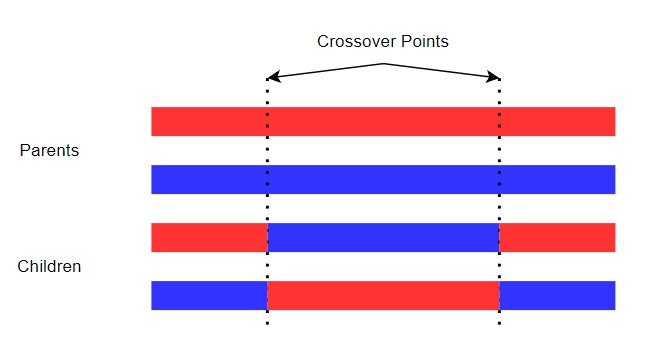
\includegraphics[height=1.5in,width=3in]{2Point}
\caption{Two Point Crossover}
\label{fig:2Point}
\end{figure}
\item[Uniform Crossover] randomly selects which parent's alleles will be copied for each gene. In our experiments, the probability for each parent to be selected is equal. \cite{Belfiore1998}
\end{description}


\subsubsection{Mutation}
Mutation affects the newly made child individuals and introduces new genetic material to the search space. This allows the population to move to new areas in the search space. A mutation rate parameter is used to determine the probability of the operator taking effect.  We implemented and tested the following operators:
\begin{description}
\item[Swap Mutation] randomly chooses two genes in the individual and swaps their alleles. The chance of mutation occuring is per individual.\cite{Mutation}
\item[Inverse Mutation] randomly selects two positions in the genome and inverts the position of all genes between these positions. The chance of mutation occuring is per individual. \cite{Mutation}
\item[Floating Point Mutation] changes the values of a gene by a set value with an equal chance of the value being added or subtracted. The chance of mutation occuring is per gene. The implementation of this was provided in the coursework.
\end{description}

\subsubsection{Replacement}
Replacement is the mechanism by which new child individuals replace existing members in the population.
\begin{description}
\item[Replace Worst] replaces the lowest fitness members of the population with the new child individuals, regardless of the child's fitness. The implementation of this was provided in the coursework
\item[Replace Worst Parent] replaces a parent individual with the new child individual, only if the child is more fit.
\item[Tournament Replacement] selects t individuals from the population and selects the least fit individual to be replaced by the child solution, if the child solution is more fit than the least fit in the tournament.

\end{description}

\subsection{Neural Network Parameters}
Parameters that can be changed are the minimum and maximum values of the weights, number of hidden nodes and the activation function.

\subsubsection{Minumum and Maximum Values}

\subsubsection{Hidden Nodes}
We note that the number of hidden nodes directly affects the number of genes present in an individual. In short, the less information a gene holds compared to the totality of the individual, the less likely it's alteration will create a meaningful exploration effect. Therefore as we increase the number of hidden nodes, we should ensure that our mutation operators operate per gene and not per individual. It is for this reason that we expect that the "Swap" Mutation operator to hinder fitness at higher hidden node values.
\subsubsection{Activation Function}
Provided by default  is a hyperbolic tangent activiation function. In addition to this, we have chosen to implement an arc tangent activation function and a softsign activation function.

\subsection{Notes}
Runtime is not considered a limiting factor in our evaluation.
\section{Experiments \& Analysis}
All results presented are a mean average from ten runs. Unless otherwise specified, all experiments were run with the following setup which was taken from a known good solution discovered during development that had a test data fitness of 0.05.

\begin{center}
\begin{tabular} {|c|c|}
\hline
Operators & Chosen Method \\
\hline
Selection & Tournament Selection \\
Recombination & Two Point Crossover \\
Mutation & Standard \\
Replacement & Worst \\
Activation & TanH \\
\hline
\end{tabular}
\end{center}
\begin{center}
\begin{tabular} {|c|c|}
\hline
Parameters & Values \\
\hline
Hidden Nodes & 10 \\
Min Gene & -3.0 \\
Max Gene & 3.0 \\
Pop Size & 200 \\
Generations & 20000 \\
Tournament Size & 50 \\
Mutation Rate & 0.5 \\
Mutation Change & 1.0 \\

\hline

\end{tabular}
\end{center}

\subsection{Operators}
\subsubsection{Selection}
Tournament Selection

\subsubsection{Mutation}
We find that the standard mutation operator provided worked best. The issue presented by "Swap" and "Inverse" mutation is that they do not introduce new genetic material. Changing the positions of the genetic values allows the search to expand into new environments but these environments are limited to values that already exist in the solution preventing true freedom to explore the search space. We suspect that a combination of "Swap"/"Inverse" and standard mutation could work well but were unable to test this under the scope of this project.

\subsection{Parameters}
\subsubsection{Hidden Nodes}
In this experiment, we alter the number of hidden nodes in the neural network, and therefore the number of genes in an individual, in a step of 2 less than and more than our default value of 10.

\subsection{Activation Function}


\begin{center}



\end{center}

\subsection{Analysis}

\section{Conclusions}
We believe that we have found a near optimal solution that performs extremely well in a variety of situations, achieving a training set fitness of 0.00863 and a test set fitness of 0.00946, rounded to five decimal places. Moreover, we achieve a fitness of 0.01454 on the "Go Nuts" set of data demonstrating the flexibility of our best solution. The operators and parameters are listed below:

\begin{center}
\begin{tabular} {|c|c|}
\hline
Operators & Chosen Method \\
\hline
Selection & Tournament Selection \\
Recombination & Two Point Crossover \\
Mutation & Standard \\
Replacement & Worst \\
\hline
\end{tabular}
\end{center}


\vspace{1em}
\begin{center}

\begin{tabular} {|c|c|}
\hline
Parameters & Values \\
\hline
Hidden Nodes & 12 \\
Min Gene & -3.0 \\
Max Gene & 3.0 \\
Pop Size & 200 \\
Generations & 20000 \\
Tournament Size & 50 \\
Mutation Rate & 0.5 \\
Mutation Change & 1.0 \\
\hline

\end{tabular}
\end{center}

Due to the high number of genes (111)  in our optimal solution, the generated weights are included as an addendum to the report.

\section{Future Work}




\bibliographystyle{ACM-Reference-Format}
\bibliography{bib} 


\end{document}
